\documentclass{article}

\PassOptionsToPackage{numbers, compress}{natbib}
\usepackage[preprint]{neurips_2026}

\usepackage[utf8]{inputenc}
\usepackage[T1]{fontenc}
\usepackage{hyperref}
\usepackage{url}
\usepackage{booktabs}
\usepackage{amsfonts}
\usepackage{amsmath}
\usepackage{amssymb}
\usepackage{nicefrac}
\usepackage{microtype}
\usepackage{xcolor}
\usepackage{graphicx}
\usepackage{multirow}
\usepackage{array}
\usepackage{enumitem}
\usepackage{float}

\newcommand{\softas}{\textsc{Soft-AS PPO}}
\newcommand{\cppo}{\textsc{C-PPO}}
\newcommand{\profitppo}{\textsc{Profit PPO}}
\newcommand{\E}{\mathbb{E}}

\title{AS-Regularized Deep Market Making without\\ Hybrid Reward Shaping}

\author{%
  Pierre Roth\thanks{Corresponding author. Code and configuration files are available at \url{https://github.com/pierre-roth/mlfcs-gapa}.} \\
  Department of Computer Science\\
  ETH Z\"urich\\
  \texttt{pierre.roth@inf.ethz.ch} \\
  \And
  Anja Petric \\
  Department of Mathematics\\
  ETH Z\"urich \\
  \texttt{apetric@ethz.ch} \\
  \AND
  Amine Benjelloun Touimi \\
  Department of Computer Science\\
  ETH Z\"urich \\
  \texttt{abenjelloun@ethz.ch} \\
  \And
  Ghali Berbich \\
  Department of Computer Science\\
  ETH Z\"urich \\
  \texttt{gberbich@ethz.ch} \\
}

\begin{document}

\maketitle

\begin{abstract}
Deep reinforcement-learning market makers are often steered by hybrid rewards that combine transformed profit-and-loss, trade incentives, and inventory penalties. These terms encode reasonable trading preferences, but their coefficients interact indirectly and make the resulting quoting policy hard to interpret or recalibrate. We revisit the Attn-LOB / C-PPO market maker of \citet{guo2023mm} and replace its hybrid reward with marked-to-market profit plus a soft action-space regularizer toward a per-stock Avellaneda--Stoikov (AS) teacher fitted on training data. The teacher supplies an interpretable quoting prior, while PPO remains able to deviate from it when the data support a different quote. On a synthetic benchmark shaped to the original experimental setup, \softas{} improves mean PnL from $60.07$ for reward-shaped \cppo{} and $65.67$ for \profitppo{} to $75.17$. In paired stock--seed comparisons, this corresponds to raw-PnL gains of $15.10$ over \cppo{} ($95\%$ CI $[9.19,21.01]$, $p=8.1\times10^{-5}$) and $9.50$ over \profitppo{} ($95\%$ CI $[5.45,13.56]$, $p=1.9\times10^{-4}$). It also outperforms directly executing the fitted AS teacher and reduces the mean action gap to the teacher from about $0.47$ for the controls to $0.23$. The behavioural change is visible: \softas{} quotes tighter and fills more orders, but carries more inventory and is more exposed to latency. These results support AS regularization as a cleaner and more inspectable alternative to hybrid reward shaping on this controlled benchmark, while leaving real-data evaluation, costs, market impact, and latency-aware calibration as necessary next steps.
\end{abstract}

\section{Introduction}

Market making is the problem of continuously quoting bid and ask limit orders to earn the spread while managing inventory risk \citep{stoll1989,odhara1998}. A modern limit order book (LOB) is high-dimensional, noisy, and fast-moving, so recent work uses deep reinforcement learning (RL) to learn quoting policies directly from LOB state. The Attn-LOB / C-PPO agent of \citet{guo2023mm} is a strong example: a convolutional-attention encoder reads a rolling LOB window and PPO emits continuous bid/ask quote parameters.

The agent's behaviour, however, is largely determined by a hand-designed reward. The original C-PPO reward adds three heuristic terms: dampened PnL, trading PnL, and an inventory penalty:
\begin{equation}
R_t
= \underbrace{\Delta\mathrm{PnL}_t-\max(0,\eta\Delta\mathrm{PnL}_t)}_{\text{dampened PnL}}
+ \underbrace{X_{t,v}(p_{m,t}-X_{t,p})}_{\text{trading PnL}}
- \underbrace{\zeta \mathrm{Inv}_t^2}_{\text{inventory penalty}} .
\label{eq:hybrid}
\end{equation}

Each term encodes a sensible intention, e.g. suppress holding profits, reward fills near mid, discourage large positions, but the encoding is opaque. The terms are not potential-based \citep{ng1999}, so they reshape the optimal policy rather than merely accelerating learning; their coefficients ($\eta,\zeta$) interact indirectly, must be re-tuned per market, and give the designer no direct read on the quoting behaviour they induce. When such an agent quotes too tightly or carries too much inventory, the reward offers no interpretable knob with which to correct it.

We ask whether the behavioural prior can instead come from a calibrated classical model, expressed where it is easiest to inspect: the action itself. We keep the marked-to-market profit as the economic reward and add a soft regularizer that pulls the learned continuous action toward a fitted Avellaneda--Stoikov (AS) teacher \citep{avellaneda2008}:
%The environment reward is pure profit, while the behavioural prior comes from Avellaneda--Stoikov (AS), a classical market-making model that gives an interpretable reservation price and spread from inventory, volatility, time remaining, risk aversion, and liquidity \citep{avellaneda2008}. Instead of copying AS, we regularize the learned continuous action toward a fitted AS teacher:
\begin{equation}
J(\pi)
= \E_{\pi}\!\left[\sum_t \Delta\mathrm{PnL}_t
- \lambda \left\lVert a^\pi_t-a^{\mathrm{AS}}_t \right\rVert_2^2 \right].
\label{eq:softas}
\end{equation}
The AS term is part of the training objective, but the economic reward being optimized is ordinary marked-to-market profit. We do not present this as a way to escape objective design; it is a soft control-prior regularizer, a domain instance of pulling a deep policy toward a fixed policy prior in action space \citep{cheng2019control}, and it changes what the agent optimizes just as the hybrid reward does. The difference is where the design lives. Rather than spreading the designer's intent across reward coefficients that interact indirectly, we concentrate it in a single object: an Avellaneda--Stoikov teacher whose parameters $\gamma$ and $\kappa$ carry economic meaning and can be calibrated per stock, with one weight $\lambda$ setting how hard the policy is held to it. Because the policy and the teacher emit actions in the same normalized space, we can also measure the gap between them directly, and so check whether the prior is actually shaping quotes rather than reading that off terminal PnL.

%Coupling AS with RL is not itself new, but the coupling matters. \citet{falcesmarin2022}, for example, have an RL network adjust AS's risk-aversion parameter and let AS produce the quotes; the learned component tunes the classical model. We do the opposite: the learned policy quotes, and AS serves only as a soft target it is free to leave when the data warrant. Otherwise we keep the agent of \citet{guo2023mm} intact (the encoder, simulator, action space, and PPO training are unchanged) and vary only how the behavioural prior enters.



%\paragraph{Contributions.}
%We formulate AS guidance as a soft action-space regularizer for continuous-action PPO market making, calibrate one AS teacher per stock from the training window, and keep the extension code separated from the paper-replication pipeline. The experiments use a matched synthetic benchmark following the original paper's stock/day/episode/action structure, with five PPO seeds for \softas{}, \cppo{}, and \profitppo{} on three synthetic stocks. We also regenerate the original-style analyses--performance by stock, latency, attention, and decision traces--for the proposed method, and add teacher-action divergence diagnostics.

\paragraph{Contributions.}
\begin{itemize}[leftmargin=1.4em,itemsep=2pt,topsep=2pt]
\item We formulate AS guidance as a soft control-prior regularizer for continuous-action PPO market making, replacing the hand-crafted hybrid reward of Eq.~\eqref{eq:hybrid} with a profit objective plus an interpretable, calibrated action prior.
\item We calibrate one AS teacher per stock from the training window, producing a behavioural prior that is inspectable, loggable, and steerable through economically meaningful knobs ($\gamma,\kappa,\lambda$).
\item On a matched synthetic replication of \citet{guo2023mm} with five seeds per stock, we show that \softas{} improves PnL and Sharpe over both reward-shaped \cppo{} and a profit-only control, and we add teacher-divergence, latency, and decision-trace diagnostics that show the prior steers quoting behaviour directly and identify failure modes.
\end{itemize}

\section{Related work}
\label{sec:related}

Classical market-making models derive quotes by balancing spread capture and inventory risk. In the AS model, with inventory $q$, mid-price $s$, volatility $\sigma$, risk aversion $\gamma$, liquidity $\kappa$, and horizon $T$, the reservation price and total spread are
\begin{equation}
r(s,q,t)=s-q\gamma\sigma^2(T-t),
\qquad
\delta^a+\delta^b=\gamma\sigma^2(T-t)+\frac{2}{\gamma}\log\!\left(1+\frac{\gamma}{\kappa}\right).
\label{eq:as}
\end{equation}
This structure is interpretable but depends on assumptions about price and arrival processes \citep{gueant2013}. Deep LOB models such as DeepLOB and related architectures learn representations directly from order-book tensors \citep{zhang2019deeplob,tsantekidis2020,ntakaris2019}, and RL market makers have used handcrafted state, discrete actions, and model-free policies \citep{lim2018,spooner2018,zhong2020,sadighian2019,gasperov2021}. \citet{guo2023mm} combine an Attn-LOB encoder with a continuous, AS-like action space and the hybrid reward in Eq.~\eqref{eq:hybrid}, trained with PPO \citep{schulman2017ppo}; we keep their encoder, simulator, action space, and training setup, and change only how the behavioural prior enters.

\paragraph{Regularizing a learned policy toward a prior.}
Keeping the profit reward while penalizing departures from a fixed action-space prior is a standard device in reinforcement learning. The closest precedent is \citet{cheng2019control}, who regularize a deep policy toward a control prior using a weight $\lambda$ that is adapted over training, and show that the regularized policy approximately preserves the prior's control-theoretic stability guarantees while reducing the variance of the policy gradient. Our penalty admits the same bias--variance reading: the AS teacher supplies structure where the data are uninformative, and $\lambda$ governs how far the policy may move away from it. Comparable constraints appear in offline RL, where the policy is tied to a behaviour prior to curb value over-estimation \citep{fujimoto2019bcq}, and in residual policy learning, where a learned term is added on top of a fixed controller \citep{silver2018residual}. What is new here is not the regularizer, which is shared across these settings, but the prior it pulls toward: a per-stock Avellaneda--Stoikov model whose parameters $\gamma$ and $\kappa$ are economically meaningful and can be calibrated and stress-tested, in place of a generic KL or proximity term.

\paragraph{Coupling AS with learning.}
Combining AS with RL is not itself new; what differs is the direction of the coupling. \citet{falcesmarin2022} have a network set AS's risk-aversion parameter and let AS produce the quotes, so learning tunes the classical model from within. We reverse this: the policy quotes directly, and AS enters only as a target it may leave when the data warrant. The classical model therefore supplies a behavioural prior rather than the quoting rule.


\section{The replicated agent}
\label{sec:replicated}


We build on the Attn-LOB / \cppo{} market maker of \citet{guo2023mm}, which has four parts: an encoder that reads the LOB, an action space that turns network outputs into quotes, a reward that defines good market making, and a replay simulator for training and evaluation. We keep all four and change only how the behavioural prior is supplied; full reproduction details are in Appendix~\ref{app:data}.

%The agent we build on has four components: an encoder that reads the LOB, an action space that maps network outputs to quote prices, a reward signal that defines good market making, and a replay simulator for training and evaluation. We retain all four from \citet{guo2023mm} and modify only the reward; full reproduction details are in Appendix~\ref{app:data}.

\paragraph{State and encoder.} The agent observes a rolling window of
$T\!=\!50$ LOB snapshots, each a $40$-dimensional vector of the top-ten
ask and bid prices and volumes. The Attn-LOB encoder reads this $50\times40$ tensor with convolutional filters, an Inception block, and a multi-head self-attention layer: the
convolutions pick up spatial patterns across price levels within each
snapshot, while the Inception and attention layers capture temporal
dependencies across the window at multiple scales. Dynamic agent state
(inventory, remaining time, and cash or marked-to-market value) is concatenated to the encoded features. We pre-train the encoder on a three-way mid-price direction task and reuse it as the PPO feature extractor, as in the original work.


\paragraph{Continuous action space.} The policy outputs two actions
$A_1,A_2\in[0,1]$. $A_1$ sets a reservation-price bias and $A_2$ the
quoted spread:
\begin{equation}
\delta = A_1 \cdot \text{max\_bias}, \quad
p_r = p_m - \mathrm{sign}(\mathrm{Inv})\,\delta, \quad
\text{spread} = A_2 \cdot \text{max\_spread}, \quad
p_{a,b} = p_r \pm \tfrac{\text{spread}}{2}.
\label{eq:action}
\end{equation}
The agent thus quotes symmetrically around a reservation price $p_r$ that it skews against its own inventory. This is deliberately the same shape as the AS closed form of Eq.~\eqref{eq:as}: $A_1$ takes the role of the inventory-dependent reservation shift $q\gamma\sigma^2(T-t)$, and $A_2$ the role of the optimal spread $\delta^a+\delta^b$.

Both the policy and the AS model write into this same $(A_1,A_2)$ space, which is what lets AS serve as a regularization target in Section~\ref{sec:method}.

\paragraph{Reward (baseline).} %The reward-shaped baseline, which we call \cppo, uses the hybrid reward of Eq.~\eqref{eq:hybrid} with $\eta=0.5$, $\zeta=0.01$, trained with PPO. As noted in Section~1, the three reward terms are not potential-based: they reshape the optimal policy rather than merely accelerating learning. The dampening coefficient $\eta$ suppresses holding profits, the inventory penalty $\zeta$ constrains position size, and the trading PnL term encourages fills near mid. These interact in ways that are difficult to disentangle, which motivates our alternative. This baseline is our primary point of comparison.

Our primary point of comparison, \cppo{}, trains PPO on the hybrid reward of Eq.~\eqref{eq:hybrid} with the original coefficients $\eta=0.5$ and $\zeta=0.01$. As noted in the introduction, these terms are not potential-based \citep{ng1999} and reshape the optimal policy rather than merely accelerating learning. We carry the coefficients over unchanged rather than re-tuning them for this benchmark. This keeps the baseline faithful to the source, and the difficulty of re-tuning such coupled terms for each new market is itself part of what motivates moving the prior out of the reward.


\paragraph{Simulator.} A replay simulator fills the agent's quotes
only when the recorded stream trades through the quoted price. There
is no market impact and no transaction cost; the agent may run long or short and is liquidated at the end of each $2000$-event episode. The simulator is identical for every method, so within-benchmark comparisons are fair. It is not, however, neutral across quoting styles: with no spread to pay and no impact to absorb, a frictionless tape rewards tight, high-participation quoting and so flatters more aggressive policies. Absolute PnL should therefore be read as a benchmark quantity rather than a live-trading estimate, and the cross-method ranking should be weighed alongside the inventory and latency costs we report in Section~\ref{sec:results}. This mirrors the small-order
assumption of the original work.

\section{AS-regularized PPO}
\label{sec:method}

We change only the training objective of the agent in Section~\ref{sec:replicated}: it still optimizes marked-to-market profit, but we add a soft penalty pulling each quoting action toward a fitted Avellaneda--Stoikov teacher. Concretely, the per-step reward is

\begin{equation}
r_t = \Delta\mathrm{PnL}_t - \lambda\,\bigl\lVert a^\pi_t - a^{\mathrm{AS}}_t \bigr\rVert_2^2 ,
\label{eq:stepreward}
\end{equation}
and PPO maximizes the resulting return $J(\pi)=\E_\pi[\sum_t r_t]$, which is Eq.~\eqref{eq:softas}. The penalty acts on the action sampled during rollout collection, so it is part of the reward the policy optimizes rather than a separate supervised loss on the network. This is what we mean by a control-prior regularizer: it modifies the objective, like the hybrid reward, but through a single interpretable target instead of several hand-set coefficients.

\paragraph{The AS teacher.}
The teacher converts the AS closed form of Eq.~\eqref{eq:as} into the same normalized $(A_1,A_2)$ coordinates the policy uses in Eq.~\eqref{eq:action}. Given inventory $q$, a volatility estimate $\hat\sigma_t$, and time-to-close $T-t$,
\begin{equation}
a^{\mathrm{AS}}_t
= \Bigl(
\operatorname{clip}\!\Bigl(\tfrac{|q|\,\gamma\,\hat\sigma_t^2\,(T-t)}{\text{max\_bias}},\,0,\,1\Bigr),\;
\operatorname{clip}\!\Bigl(\tfrac{\delta^a+\delta^b}{\text{max\_spread}},\,0,\,1\Bigr)
\Bigr),
\qquad
\delta^a+\delta^b = \gamma\hat\sigma_t^2(T-t) + \tfrac{2}{\gamma}\log\!\bigl(1+\tfrac{\gamma}{\kappa}\bigr).
\label{eq:teacher}
\end{equation}
The first coordinate matches the inventory-dependent reservation shift of Eq.~\eqref{eq:action} and the second the optimal spread; clipping into $[0,1]$ keeps the teacher inside the policy's action range. The sign of the bias is supplied by $\operatorname{sign}(\mathrm{Inv})$ in Eq.~\eqref{eq:action}, so the teacher carries only its magnitude $|q|$. Once $(\gamma,\kappa)$ are fixed and $\hat\sigma_t$ is read from the state, the teacher is a deterministic function of the agent's situation and adds no learnable parameters.

\paragraph{Calibration.}
We fit one teacher per stock from the training window only. The liquidity parameter $\kappa$ is estimated from the mean level-one half-spread, giving $\kappa = 125.2,\ 23.9,\ 83.8$ for stocks 000001, 000858, and 002415. For risk aversion we use a fixed low-risk value $\gamma = 0.025$ for the reported policy; a volatility-fitted $\gamma$ and a higher-risk teacher are evaluated as controls in Appendix~\ref{app:sensitivity}. The volatility term $\hat\sigma_t$ is a rolling realized-volatility estimate computed from the same LOB stream the policy sees. We freeze the calibration used at training time and reuse it at evaluation, rather than recalibrating on the test split, so the teacher cannot leak test-window information into the policy's prior.

\paragraph{Methods compared.}
We report three PPO agents that share this state, encoder, action space, and training budget, and differ only in the objective. \cppo{} is the reward-shaped baseline of Section~\ref{sec:replicated}. \profitppo{} drops the hybrid terms and trains on profit alone ($\lambda=0$ in Eq.~\eqref{eq:stepreward}), isolating the effect of removing the old reward. \softas{} adds the AS regularizer with $\lambda=0.10$ and the low-risk per-stock teacher. The three thus form a clean decomposition: \cppo{}~$\to$~\profitppo{} measures the effect of replacing the hand-crafted reward with pure profit, and \profitppo{}~$\to$~\softas{} measures what the calibrated prior adds on top. Hard AS constraints, behavioural-cloning warm starts, a direct-AS teacher policy, and the $\lambda$ sweep are appendix-only controls (Appendix~\ref{app:sensitivity}).



\section{Experimental setup}
\label{sec:setup}

\paragraph{A synthetic benchmark.}
The original Shenzhen Stock Exchange LOB data are proprietary, so we use a synthetic event-level LOB generator that preserves the experimental shape of \citet{guo2023mm}: three stock identities, top-ten book levels, stable intraday windows, ten training days, eleven test days, and 2000-event episodes.
Each instrument has its own base price and generated training/test days; a latent fair value moves through stable, trending, and volatile regimes while the generator builds the surrounding book, trade stream, and market-order flow. The simulator replays this stream and fills the agent's quotes only when recorded trades cross the quote. There is no market impact and no transaction cost. The benchmark is useful for controlled comparisons and debugging because every method faces the same synthetic tapes, but it remains a proxy for the proprietary data used in the original paper. Appendix~\ref{app:data} gives the generator details.

\paragraph{Training protocol.}
Following the original code, we train one policy per stock rather than a single shared cross-stock policy. All three agents (Section~\ref{sec:method}) use the same state, encoder, action space, trade granularity, train/test split, and 400k PPO steps, and differ only in the objective. The main comparison runs five PPO seeds per stock for each of \cppo{}, \profitppo{}, and \softas{}, giving 15 stock--seed units per method. The regularizer weight $\lambda$ and the per-stock teacher were selected in an earlier sweep (Appendix~\ref{app:sensitivity}); the final comparison reports five seeds per stock for the selected setting.

\paragraph{Metrics.}
Our main performance metric is marked-to-market PnL, $\mathrm{PnL}=V_T-V_0$, measured over an episode. Because the three stocks have different price and spread scales, we also report spread-normalized PnL, $\mathrm{ND\text{-}PnL}=\mathrm{PnL}/(\overline{s}+10^{-7})$, where $\overline{s}$ is the mean quoted spread. ND-PnL is useful for checking whether an effect is only a price-scale artifact; PnL remains the quantity optimized by the profit-based methods. We also report Sharpe computed on event-to-event marked-value increments $\Delta V_t$ as $\sqrt{n}\,\overline{\Delta V}/\mathrm{sd}(\Delta V)$ without annualization, and behavioural quantities (mean absolute inventory, mean quoted spread, fills per episode).

\paragraph{Significance.}
Paired tests compare two agents on the same stock and seed before pooling differences across stocks. We report the mean paired PnL difference, a $95\%$ confidence interval, and the paired win rate over the 15 units. Because the units cluster in three stocks rather than 15 independent draws, we read the pooled test alongside the per-stock breakdown in Appendix~\ref{app:tables} rather than treating the 15 as independent.


% Paired tests use stock--seed units, not individual episodes.

\newpage
\section{Results}
\label{sec:results}

\begin{table}[t]
\centering
\small
\caption{Five-seed matched comparison. Values average 15 stock--seed units per method. PnL and Sharpe include standard errors across those units.}
\label{tab:main}
\begin{tabular}{lcccccc}
\toprule
Method & PnL ($\pm$SE) & ND-PnL & Sharpe ($\pm$SE) & Abs. inv. & Spread & Fills \\
\midrule
\softas{} & $\mathbf{75.17}\pm22.06$ & $\mathbf{1223.9}$ & $\mathbf{2.54}\pm0.44$ & $54.2$ & $0.0468$ & $511.7$ \\
\profitppo{} & $65.67\pm22.51$ & $1010.5$ & $2.29\pm0.42$ & $26.6$ & $0.0551$ & $437.7$ \\
\cppo{} & $60.07\pm21.38$ & $812.1$ & $2.07\pm0.51$ & $19.3$ & $0.0637$ & $333.1$ \\
Direct AS & $26.64\pm4.82$ & $462.2$ & $0.75\pm0.12$ & $157.5$ & $0.0544$ & $24.7$ \\
\bottomrule
\end{tabular}
\end{table}

\begin{figure}[t]
\centering
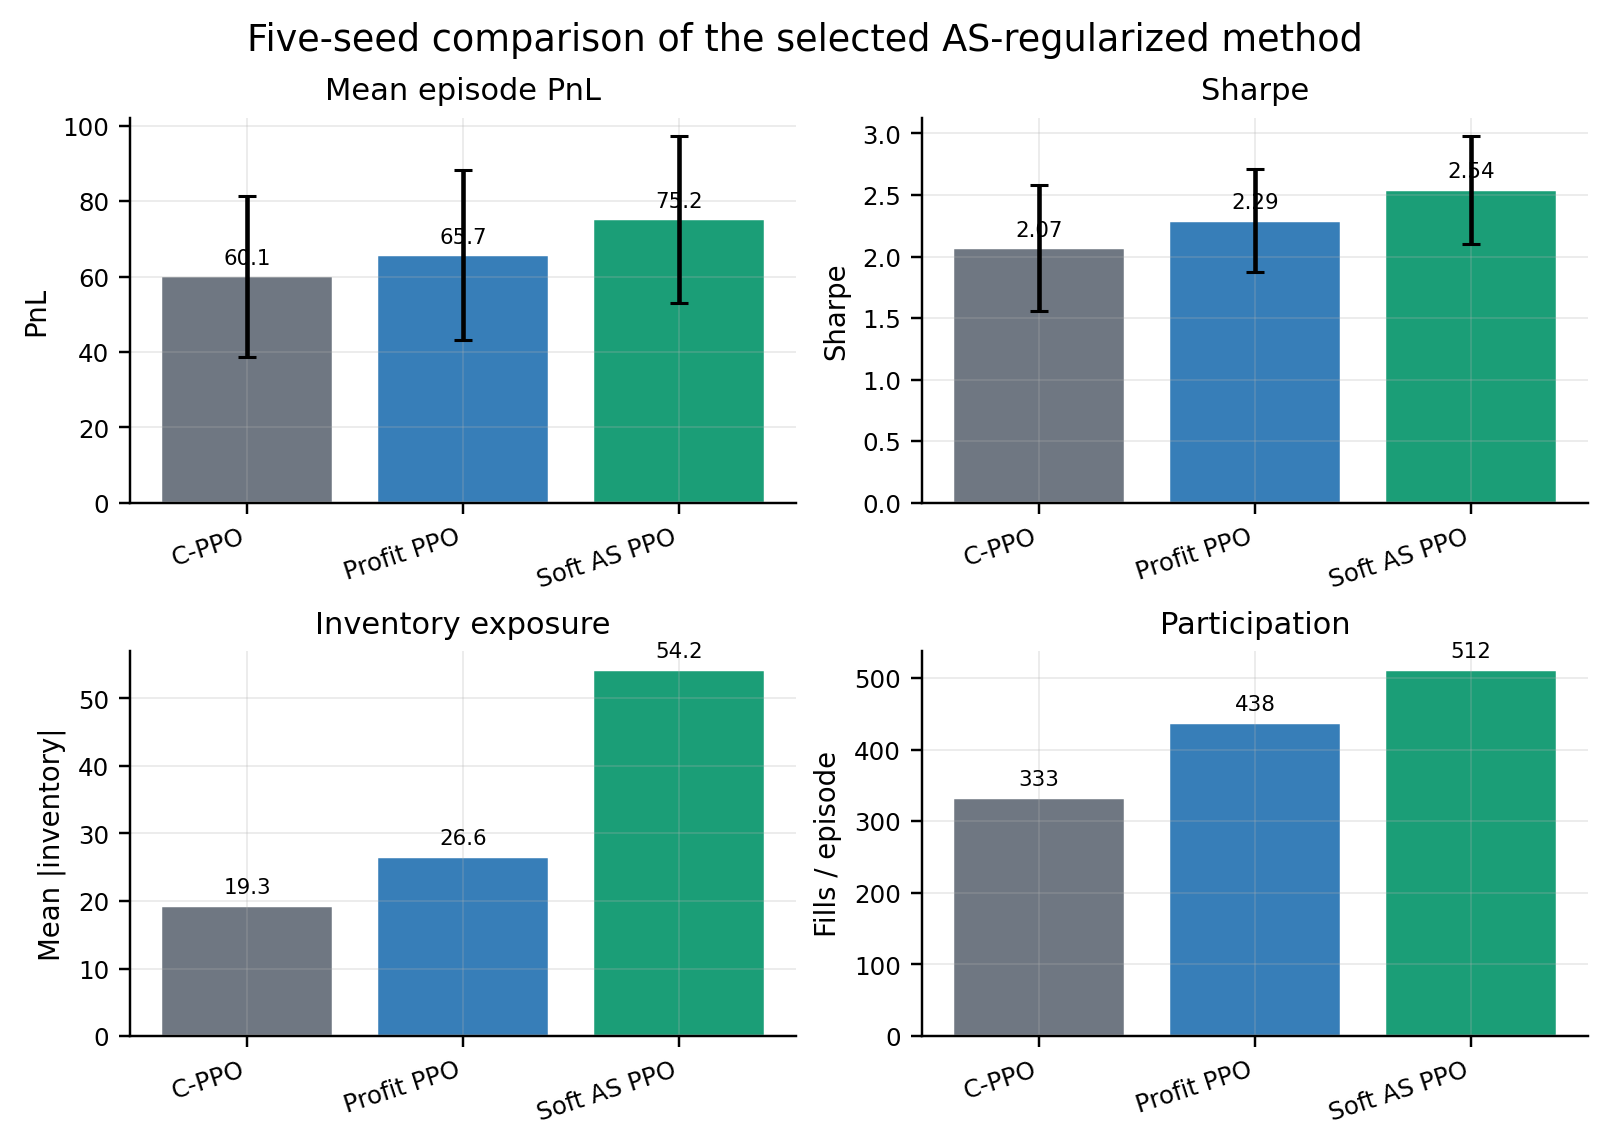
\includegraphics[width=\textwidth]{figs/fig_results_overview.png}
\caption{Headline performance and risk diagnostics over five seeds. \softas{} has the strongest ND-PnL and Sharpe, but reaches them by quoting tighter and participating more, which raises inventory exposure.}
\label{fig:overview}
\end{figure}

\subsection{Soft AS improves return over both controls}


Our primary comparison is paired PnL, because it holds the stock and seed fixed before differences are pooled. Against the reward-shaped \cppo{} baseline, \softas{} improves per-unit PnL by $15.10$ ($95\%$ CI $[9.19,21.01]$, $p=8.1\times10^{-5}$) and wins on 14 of 15 units; against \profitppo{}, which already removes the hybrid reward, it improves by $9.50$ ($95\%$ CI $[5.45,13.56]$, $p=1.9\times10^{-4}$) and again wins on 14 of 15 (Table~\ref{tab:paired}). The second comparison is the more informative one: \profitppo{} has stripped out the old reward entirely, so the gain over it is attributable to the calibrated AS prior rather than to dropping the hybrid terms.

The aggregate metrics in Table~\ref{tab:main} tell the same story. \softas{} has the highest mean PnL ($75.17$ against $60.07$ for \cppo{} and $65.67$ for \profitppo{}), and it also leads on ND-PnL ($1223.9$ vs.\ $812.1$ and $1010.5$) and Sharpe ($2.54$ vs.\ $2.07$ and $2.29$). The ND-PnL result is a useful scale check: it shows that the higher average PnL is not only a consequence of the high-price stock dominating the pooled mean.

Figure~\ref{fig:perstock} and Appendix~\ref{app:tables} break the gain down by stock: \softas{} improves over \cppo{} on the low-price stock 000001 and the mid-price stock 002415, and remains competitive on the liquid high-price stock 000858, where the profit-only control is the strongest on ND-PnL. The gain is therefore spread across stocks rather than a single-stock artifact.




\begin{table}[t]
\centering
\small
\caption{Paired raw-PnL comparisons over 15 stock--seed units. The differences are computed within stock and seed; their scale should be read together with ND-PnL and the per-stock table.}
\label{tab:paired}
\begin{tabular}{llcccc}
\toprule
Method & Baseline & $\Delta$PnL & $95\%$ CI & $p$ & Win rate \\
\midrule
\softas{} & \cppo{} & $15.10$ & $[9.19,21.01]$ & $8.1{\times}10^{-5}$ & $0.93$ \\
\profitppo{} & \cppo{} & $5.60$ & $[0.36,10.83]$ & $0.038$ & $0.73$ \\
\softas{} & \profitppo{} & $9.50$ & $[5.45,13.56]$ & $1.9{\times}10^{-4}$ & $0.93$ \\
\softas{} & Direct AS & $48.54$ & $[11.42,85.66]$ & $0.014$ & $0.80$ \\
\bottomrule
\end{tabular}
\end{table}

\begin{figure}[t]
\centering
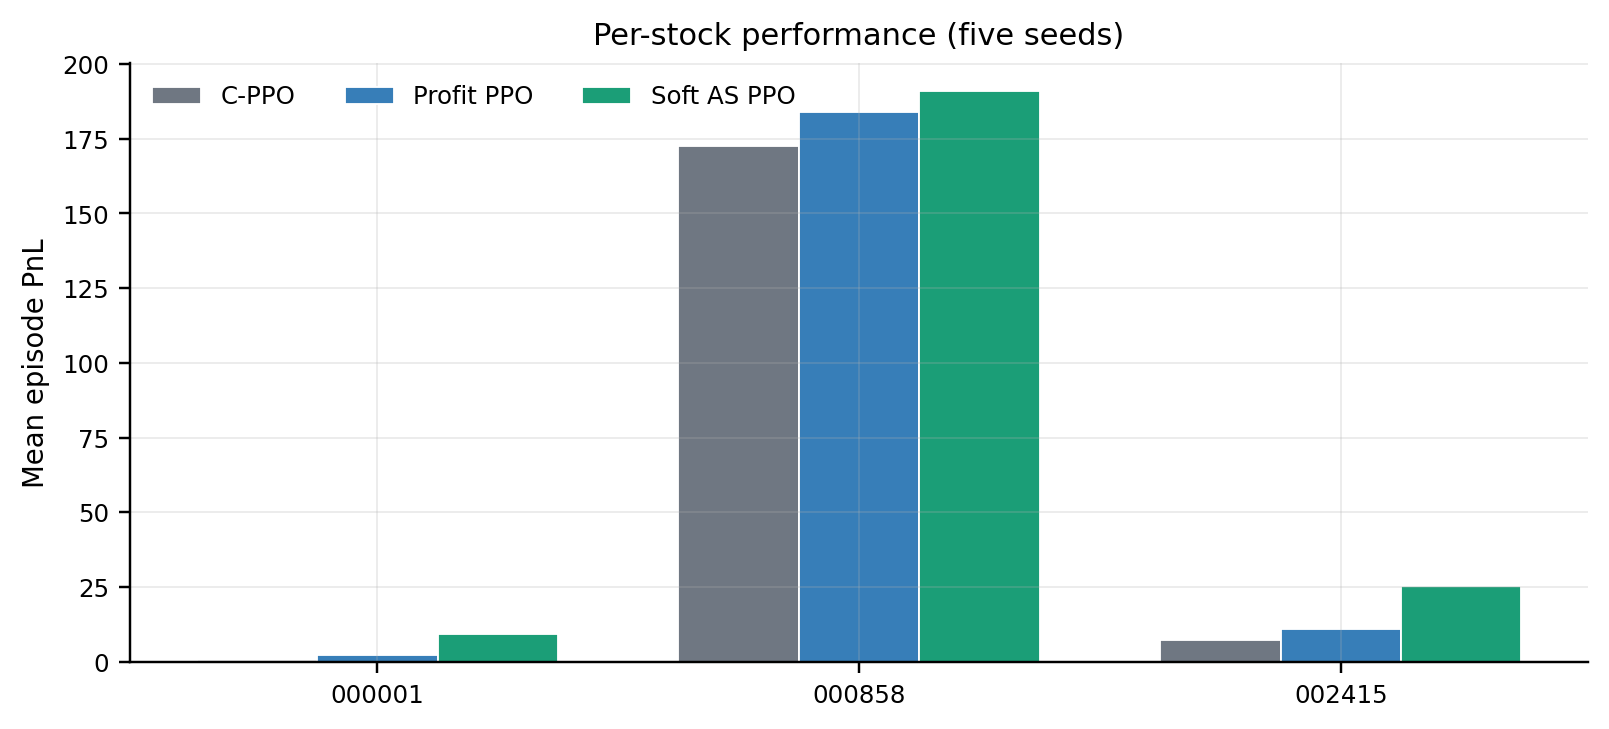
\includegraphics[width=0.96\textwidth]{figs/fig_per_stock_pnl.png}
\caption{Per-stock mean episode PnL over five seeds. The proposed method improves clearly on the low-price and mid-price stocks and remains competitive on the high-price liquid stock.}
\label{fig:perstock}
\end{figure}


\subsection{The policy departs from its teacher}
\label{sec:res-teacher}

Because \softas{} is regularized toward AS, the natural question is
whether it merely reproduces the teacher. It does not. Direct AS under
the same low-risk per-stock calibration reaches $26.64$ mean PnL,
$462.2$ ND-PnL, and $0.75$ Sharpe (Table~\ref{tab:main}). \softas{}
improves on it by $48.54$ PnL in the paired stock--seed comparison
($95\%$ CI $[11.42,85.66]$, $p=0.014$) and wins 12 of the 15 units
(Table~\ref{tab:paired}). The result is not uniform across stocks:
direct AS is competitive on the low-price stock 000001, while
\softas{} is much stronger on 000858 and 002415. The teacher-divergence
diagnostics in Section~\ref{sec:res-behaviour} are consistent with this pattern:
the policy stays close to AS in action space, but the gap is not zero.
The soft prior supplies structure without forcing the policy to copy
the teacher everywhere.

\subsection{The AS prior changes behaviour directly}
\label{sec:res-behaviour}

The main advantage of AS regularization over reward shaping is inspectability: at evaluation time we can log both the policy action and the AS teacher action. Figure~\ref{fig:teacher} shows that \softas{} is substantially closer to the teacher in both quote-bias and spread coordinates. The mean L2 action gap falls from $0.468$ for \cppo{} and $0.469$ for \profitppo{} to $0.230$ for \softas{}.

\begin{figure}[t]
\centering
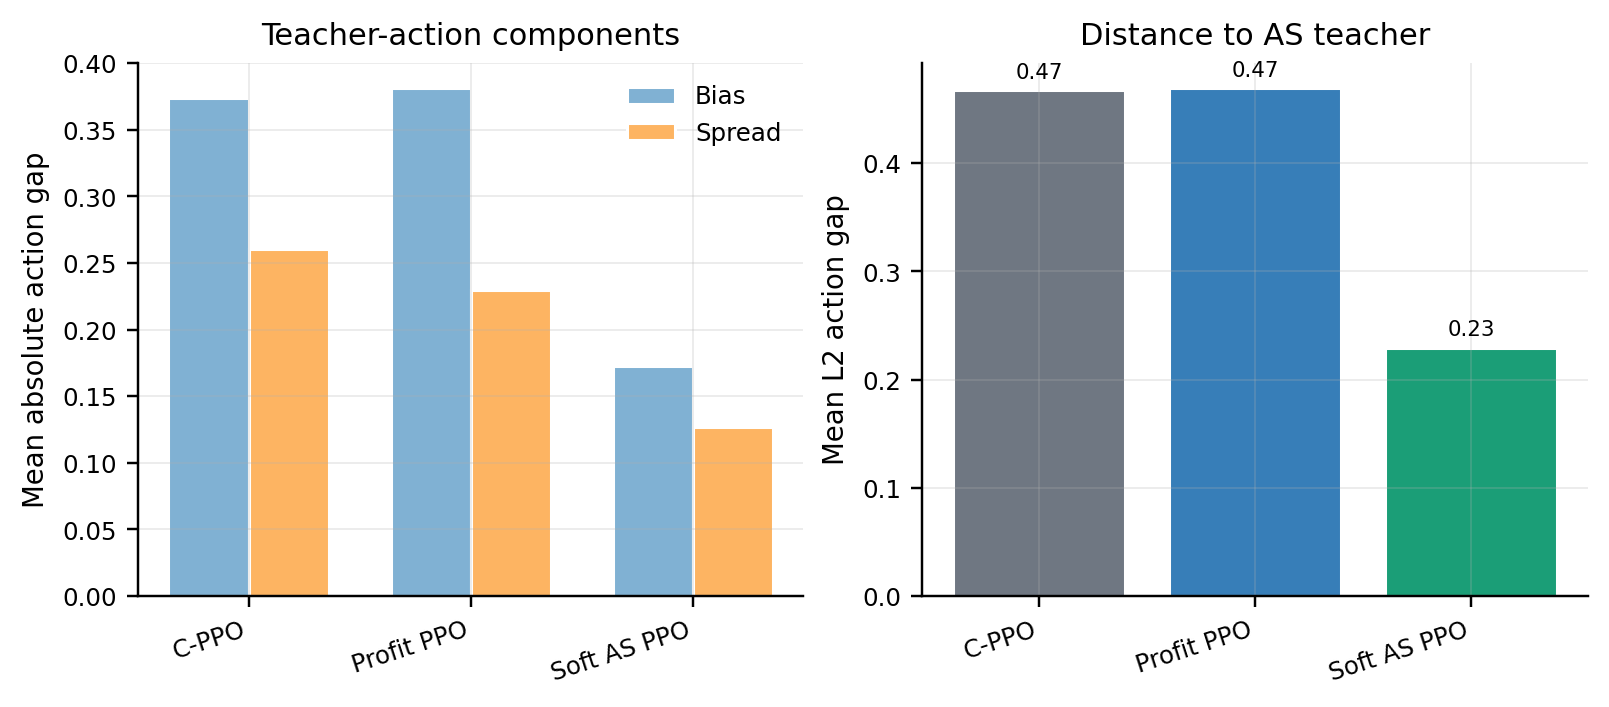
\includegraphics[width=\textwidth]{figs/fig_teacher_divergence.png}
\caption{Teacher-divergence diagnostics from saved seed-0/1/2 checkpoints. \softas{} remains much closer to the fitted AS teacher than either control, showing that the regularizer directly steers quoting behaviour rather than only changing terminal PnL.}
\label{fig:teacher}
\end{figure}

Consistent with this, in the five-seed training evaluation \softas{} has higher average inventory and more fills than both controls (Table~\ref{tab:main}). AS regularization improves the policy by making it more willing to quote, so the added return comes with a clearer inventory and latency tradeoff.


\subsection{Latency remains the main weakness}
%The original paper studied latency, so we reran an evaluation-only latency sweep for the saved seed-0/1/2 checkpoints at 1, 5, 10, 20, and 50 events. Figure~\ref{fig:latency} shows the key caveat. At low latency, \softas{} has the best return. As latency grows, all methods degrade, and the more active \softas{} policy degrades faster because stale quotes and larger inventory become costly. This is a useful stress test for the paper: it supports the low-latency result and exposes where an AS-regularized market maker needs stronger inventory or latency-aware controls.
To stress-test robustness we run an evaluation-only latency sweep on the saved checkpoints at 1, 5, 10, 20, and 50 events; the policies were trained at zero latency, so this measures how latency-naive policies degrade rather than how a latency-aware agent would behave. At low latency \softas{} has the best return. As latency grows all methods degrade, and \softas{} degrades fastest (Figure~\ref{fig:latency}): the same tight, high-participation quoting that wins at low latency becomes costly once quotes are stale and inventory is larger. This supports the low-latency result while marking exactly where an AS-regularized maker would need latency-aware or inventory-aware control.

\begin{figure}[t]
\centering
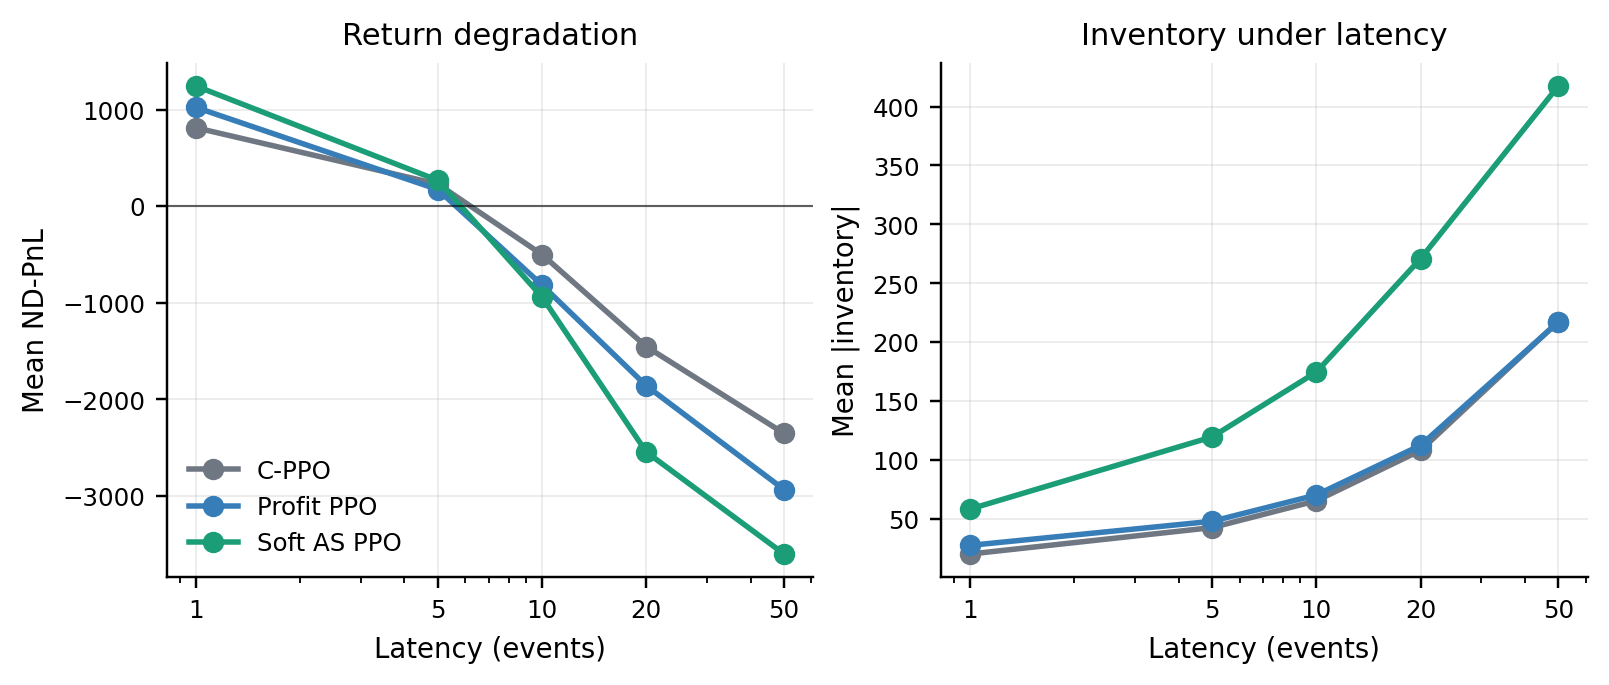
\includegraphics[width=\textwidth]{figs/fig_latency_sweep.png}
\caption{Latency sweep on saved seed-0/1/2 policies. \softas{} is best at short latency but is more exposed at high latency because it participates more and carries more inventory.}
\label{fig:latency}
\end{figure}

\subsection{Decision trace}

\begin{figure}[H]
\centering
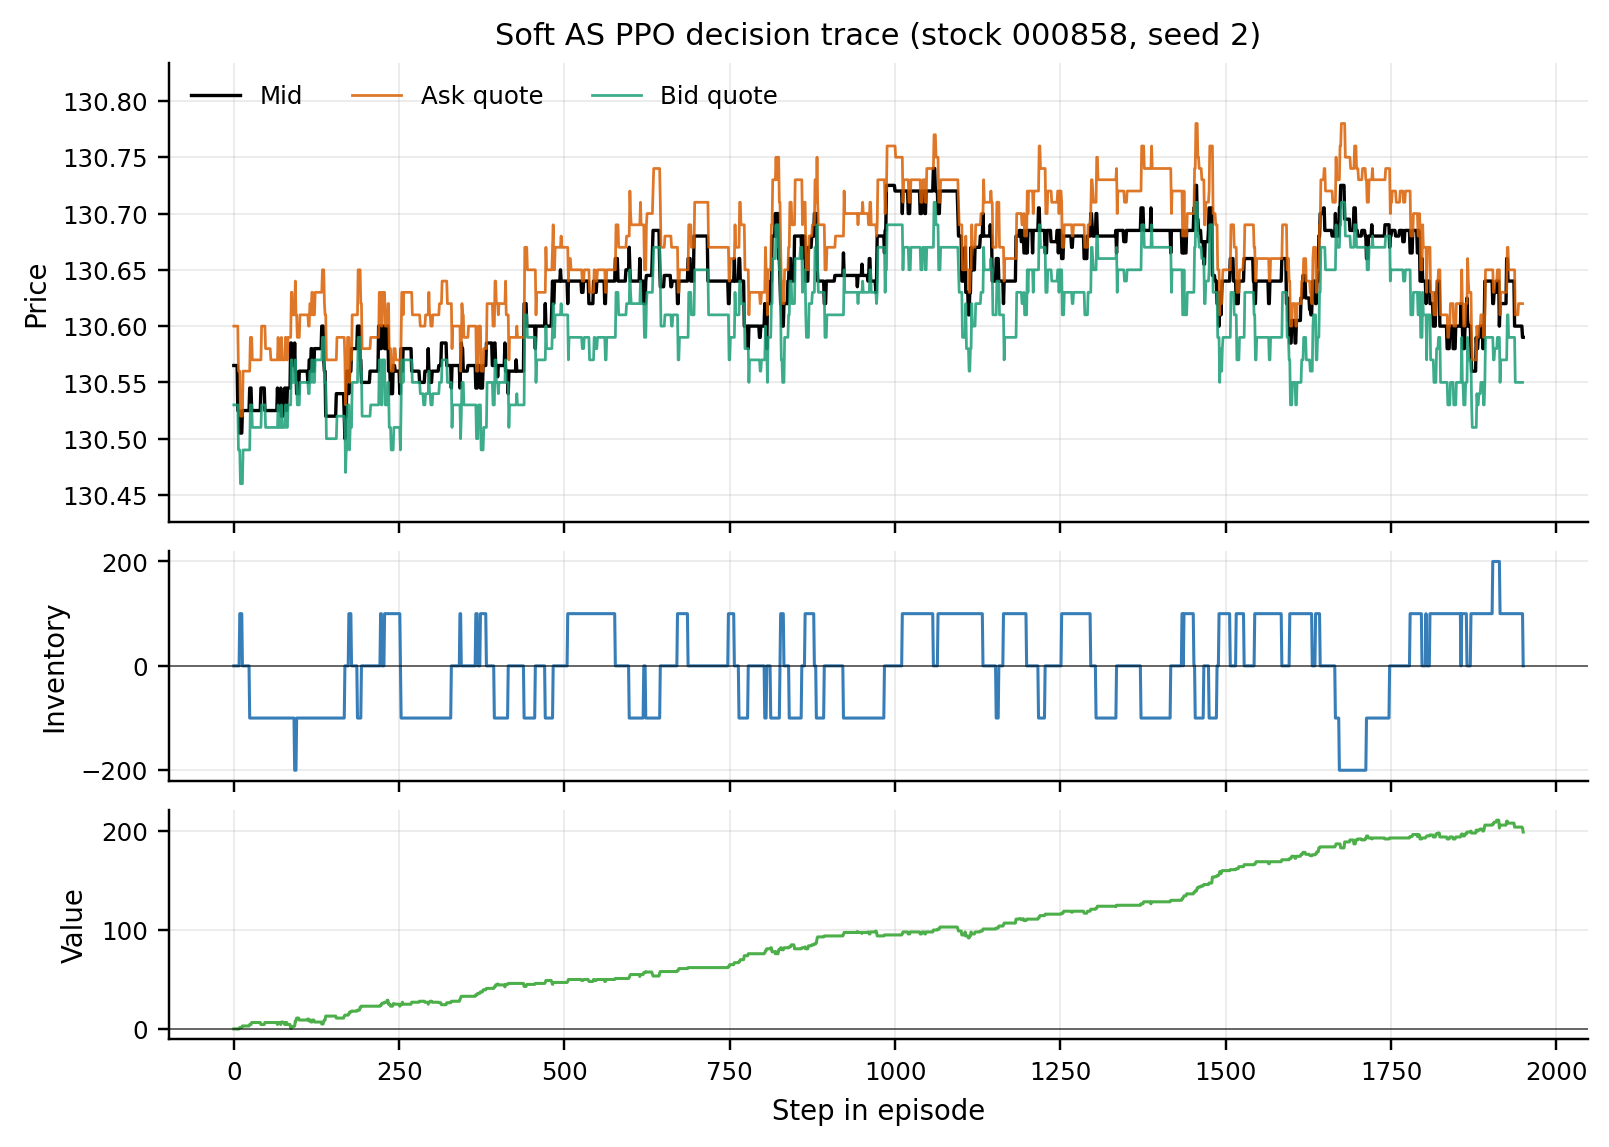
\includegraphics[width=0.92\textwidth]{figs/fig_decision_trace.png}
\caption{Decision trace for \softas{} on stock 000858, seed 2. The policy quotes actively around the mid-price, manages inventory around zero, and accumulates positive marked-to-market value over the episode.}
\label{fig:decision}
\end{figure}

Figure~\ref{fig:decision} mirrors the original paper's decision-trace diagnostic for the proposed method. It is descriptive rather than causal, but it shows that the improved policy still looks like a market maker (quoting both sides around mid and reverting inventory) rather than a sparse opportunistic trader.

\section{Discussion}
\label{sec:discussion}

\paragraph{Why the soft prior helps.} The three main methods separate the effect of the old reward from the effect of the AS prior. \profitppo{} edges out \cppo{} by a smaller and less certain margin (Table~\ref{tab:paired}), suggesting the hybrid reward was at best no help in this synthetic setting. \softas{} then beats \profitppo{} more decisively, which points to the classical teacher adding useful structure beyond the reward change. Hard AS constraints, reported in Appendix~\ref{app:sensitivity}, were weaker because clipping the policy near AS removes profitable deviations. The soft prior works better because the policy can still move away from the teacher when the data support it. The latency results reinforce this point. Active quoting helps when information is fresh, but the same behavior becomes dangerous when quotes go stale. A rigid constraint or a shaped reward that discourages
participation would completely hide this tradeoff. The soft prior makes it visible.

\paragraph{Scope and risk.}
The claim is intentionally narrow. On a paper-shaped synthetic benchmark, with per-stock policies and matched seeds, AS-regularized PPO is a more profitable and more interpretable alternative to hybrid reward shaping. The method trades more and carries more inventory, and the latency sweep shows that this matters when quotes become stale. A live or proprietary-data claim would require a real event stream, transaction costs, market impact, and stricter tail-risk constraints. The synthetic data was also designed to make spread capture learnable, with only soft adverse selection. Real markets with heavier informed
flow would likely be less kind to aggressive quoting strategies.

\paragraph{Practical value.}
Reward shaping hides design decisions inside scalar coefficients that interact indirectly. An AS action prior makes those decisions inspectable: the teacher can be calibrated, logged at evaluation time, and stress-tested, and the policy's distance from it can be measured directly (Section~\ref{sec:res-behaviour}). When the teacher is too aggressive, $\gamma$, $\kappa$, or $\lambda$ are economically meaningful knobs, which is easier to reason about than a hybrid reward whose terms trade off implicitly.

\section{Conclusion}

We revisited a reward-shaped deep market maker and replaced its hybrid
reward with a pure-profit objective plus a soft Avellaneda--Stoikov
action prior. The motivation was practical: hybrid rewards encode useful behavioural intentions but spread them across coupled coefficients that are hard to interpret, tune, and
debug when the agent misbehaves. An AS action prior replaces all of that with a single classical model whose parameters have clear economic meaning.

On a controlled synthetic replication of the original experimental
setup, \softas{} improves mean PnL from $60.07$ for reward-shaped \cppo{} and $65.67$ for a profit-only control to $75.17$
across five seeds per stock, and the gain is supported by paired tests
and the per-stock breakdown. The Sharpe ratio also
improves ($2.54$ against $2.07$ for \cppo{}), indicating that the
higher returns are not simply noisier. Teacher-divergence diagnostics
confirm that the regularizer directly steers quoting behaviour: on average, the
policy stays close to the AS teacher but moves away from it when the data reward a different quote, consistent with a policy that inherits the teacher's structure while retaining the freedom that a hard constraint would remove.

This comes with a tradeoff. \softas{} quotes tighter, fills more
often, and carries approximately three times the inventory of \cppo{}. The
latency sweep shows that this active profile degrades faster when
quotes become stale, which would matter in any deployment with
non-negligible communication or computation delays. These are direct consequences of the method's strength: a prior that encourages participation will tend to carry
more inventory risk than one that discourages it.

Several questions remain open. A state-dependent or annealed
$\lambda$ could let the agent tighten its adherence to the teacher
in volatile regimes and loosen it in stable ones. Most importantly,
evaluation on a non-proprietary real LOB stream would test whether
the AS prior remains useful when the fill process, adverse selection,
and microstructure differ from the synthetic benchmark.



\newpage
\bibliographystyle{plainnat}
\begin{thebibliography}{99}
\providecommand{\natexlab}[1]{#1}

\bibitem[Avellaneda and Stoikov(2008)]{avellaneda2008}
M.~Avellaneda and S.~Stoikov.
\newblock High-frequency trading in a limit order book.
\newblock \emph{Quantitative Finance}, 8(3):217--224, 2008.

\bibitem[Cheng et al.(2019)]{cheng2019control}
R.~Cheng, A.~Verma, G.~Orosz, S.~Chaudhuri, Y.~Yue, and J.~W. Burdick.
\newblock Control regularization for reduced variance reinforcement learning.
\newblock In \emph{ICML}, pages 1940--1949, 2019.

\bibitem[Falces Mar\'in et al.(2022)]{falcesmarin2022}
J.~Falces Mar\'in, D.~D\'iaz Pardo de Vera, and E.~L\'opez Gonzalo.
\newblock A reinforcement learning approach to improve the performance of the Avellaneda--Stoikov market-making algorithm.
\newblock \emph{PLOS ONE}, 17(12):e0277042, 2022.

\bibitem[Fujimoto et al.(2019)]{fujimoto2019bcq}
S.~Fujimoto, D.~Meger, and D.~Precup.
\newblock Off-policy deep reinforcement learning without exploration.
\newblock In \emph{ICML}, 2019.

\bibitem[Ga\v{s}perov and Kostanj\v{c}ar(2021)]{gasperov2021}
B.~Ga\v{s}perov and Z.~Kostanj\v{c}ar.
\newblock Market making with signals through deep reinforcement learning.
\newblock \emph{IEEE Access}, 9:61611--61622, 2021.

\bibitem[Gould et al.(2013)]{gould2013}
M.~D. Gould, M.~A. Porter, S.~Williams, M.~McDonald, D.~J. Fenn, and S.~D. Howison.
\newblock Limit order books.
\newblock \emph{Quantitative Finance}, 13(11):1709--1742, 2013.

\bibitem[Gu\'eant et al.(2013)]{gueant2013}
O.~Gu\'eant, C.-A. Lehalle, and J.~Fernandez-Tapia.
\newblock Dealing with the inventory risk: a solution to the market making problem.
\newblock \emph{Mathematics and Financial Economics}, 7(4):477--507, 2013.

\bibitem[Guo et al.(2023)]{guo2023mm}
H.~Guo et al.
\newblock Market making with deep reinforcement learning from limit order books.
\newblock \emph{arXiv:2305.15821}, 2023.

\bibitem[Ho and Stoll(1981)]{ho1981}
T.~Ho and H.~R. Stoll.
\newblock Optimal dealer pricing under transactions and return uncertainty.
\newblock \emph{Journal of Financial Economics}, 9(1):47--73, 1981.

\bibitem[Lim and Gorse(2018)]{lim2018}
Y.-S. Lim and D.~Gorse.
\newblock Reinforcement learning for high-frequency market making.
\newblock In \emph{ESANN}, pages 521--526, 2018.

\bibitem[Ng et al.(1999)]{ng1999}
A.~Y. Ng, D.~Harada, and S.~Russell.
\newblock Policy invariance under reward transformations: theory and application to reward shaping.
\newblock In \emph{ICML}, pages 278--287, 1999.

\bibitem[Ntakaris et al.(2019)]{ntakaris2019}
A.~Ntakaris, G.~Mirone, J.~Kanniainen, M.~Gabbouj, and A.~Iosifidis.
\newblock Feature engineering for mid-price prediction with deep learning.
\newblock \emph{IEEE Access}, 7:82390--82412, 2019.

\bibitem[O'Hara(1998)]{odhara1998}
M.~O'Hara.
\newblock \emph{Market Microstructure Theory}.
\newblock John Wiley \& Sons, 1998.

\bibitem[Sadighian(2019)]{sadighian2019}
J.~Sadighian.
\newblock Deep reinforcement learning in cryptocurrency market making.
\newblock \emph{arXiv:1911.08647}, 2019.

\bibitem[Schulman et al.(2017)]{schulman2017ppo}
J.~Schulman, F.~Wolski, P.~Dhariwal, A.~Radford, and O.~Klimov.
\newblock Proximal policy optimization algorithms.
\newblock \emph{arXiv:1707.06347}, 2017.

\bibitem[Silver et al.(2018)]{silver2018residual}
T.~Silver, K.~Allen, J.~Tenenbaum, and L.~P. Kaelbling.
\newblock Residual policy learning.
\newblock \emph{arXiv:1812.06298}, 2018.

\bibitem[Spooner et al.(2018)]{spooner2018}
T.~Spooner, J.~Fearnley, R.~Savani, and A.~Koukorinis.
\newblock Market making via reinforcement learning.
\newblock \emph{arXiv:1804.04216}, 2018.

\bibitem[Stoll(1989)]{stoll1989}
H.~R. Stoll.
\newblock Inferring the components of the bid-ask spread: theory and empirical tests.
\newblock \emph{The Journal of Finance}, 44(1):115--134, 1989.

\bibitem[Tsantekidis et al.(2020)]{tsantekidis2020}
A.~Tsantekidis, N.~Passalis, A.~Tefas, J.~Kanniainen, M.~Gabbouj, and A.~Iosifidis.
\newblock Using deep learning for price prediction by exploiting stationary limit order book features.
\newblock \emph{Applied Soft Computing}, 93:106401, 2020.

\bibitem[Zhang et al.(2019)]{zhang2019deeplob}
Z.~Zhang, S.~Zohren, and S.~Roberts.
\newblock DeepLOB: deep convolutional neural networks for limit order books.
\newblock \emph{IEEE Transactions on Signal Processing}, 67(11):3001--3012, 2019.

\bibitem[Zhong et al.(2020)]{zhong2020}
Y.~Zhong, Y.~Bergstrom, and A.~R. Ward.
\newblock Data-driven market-making via model-free learning.
\newblock In \emph{IJCAI}, pages 4461--4468, 2020.

\end{thebibliography}
\newpage
\appendix

\section*{Appendix}
\section{Synthetic benchmark}
\label{app:data}

The synthetic generator produces event-level LOB days with a latent fair-value process, bid--ask bounce, stable/trending/volatile regimes, market-order flow, and top-10 price/volume levels. Each day has $10{,}000$ raw events before stable-window filtering; downstream evaluation keeps the original paper's stable trading windows, 10:00--11:30 and 13:00--14:30. The three instruments use base prices $16.45$ (000001), $130.00$ (000858), and $35.00$ (002415), giving low-, high-, and mid-price test cases with different realized spread and volatility scales.

The generator first simulates a latent fair value on the tick grid. Regime labels change the probability and size of fair-value moves, and order-flow intensity changes with the regime. Around the fair value, the code builds ask and bid ladders with ten levels of prices and volumes, then records trades whose signs and prices can cross the agent's later quotes during replay. This gives the policy the same kind of $50\times40$ LOB tensor used by \citet{guo2023mm}, while keeping the data fully reproducible and shareable. The replay simulator has no market impact and no transaction cost, so the benchmark should be read as controlled method-comparison evidence rather than market-deployment evidence.

\section{Teacher calibration and sensitivity}
\label{app:sensitivity}

\begin{figure}[H]
\centering
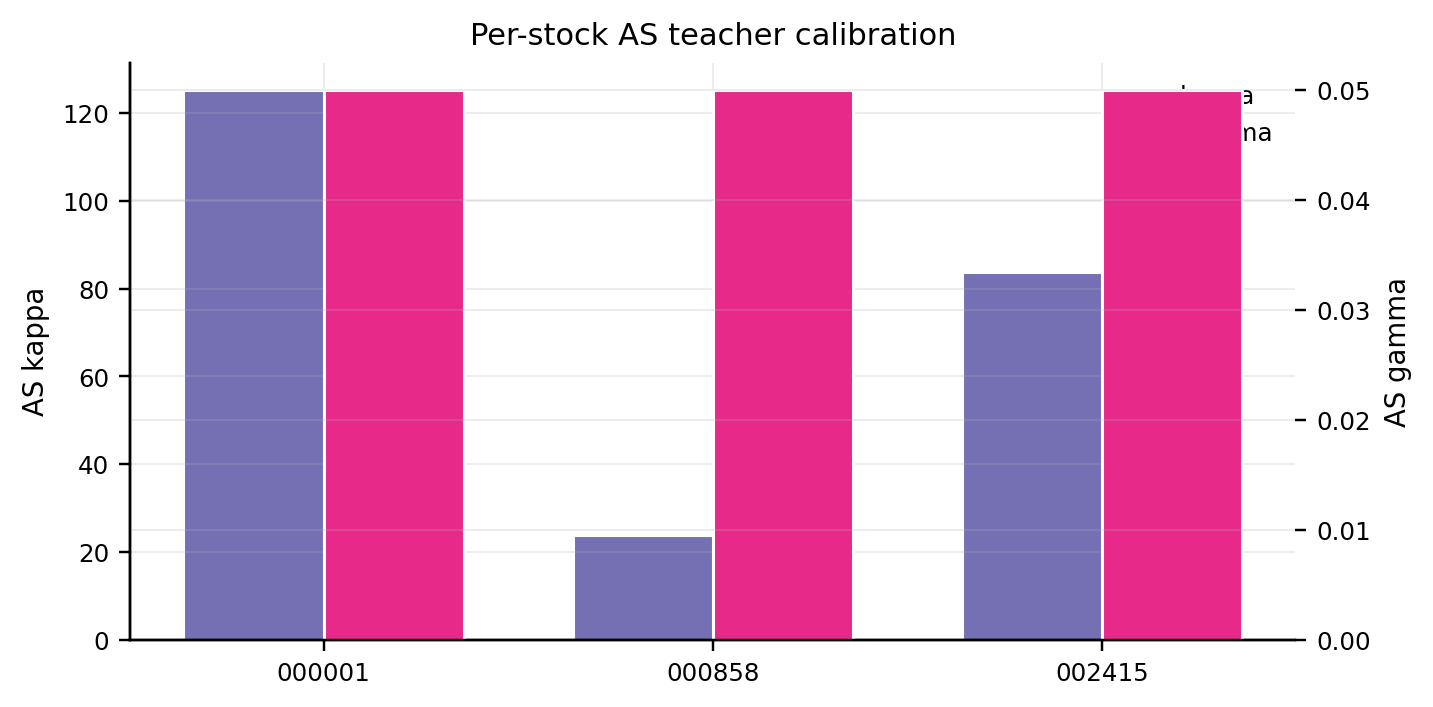
\includegraphics[width=0.78\textwidth]{figs/fig_as_calibration.png}
\caption{Per-stock AS teacher parameters used by the fitted direct-AS teacher and the AS-regularized policies.}
\label{fig:ascalib}
\end{figure}

\begin{figure}[H]
\centering
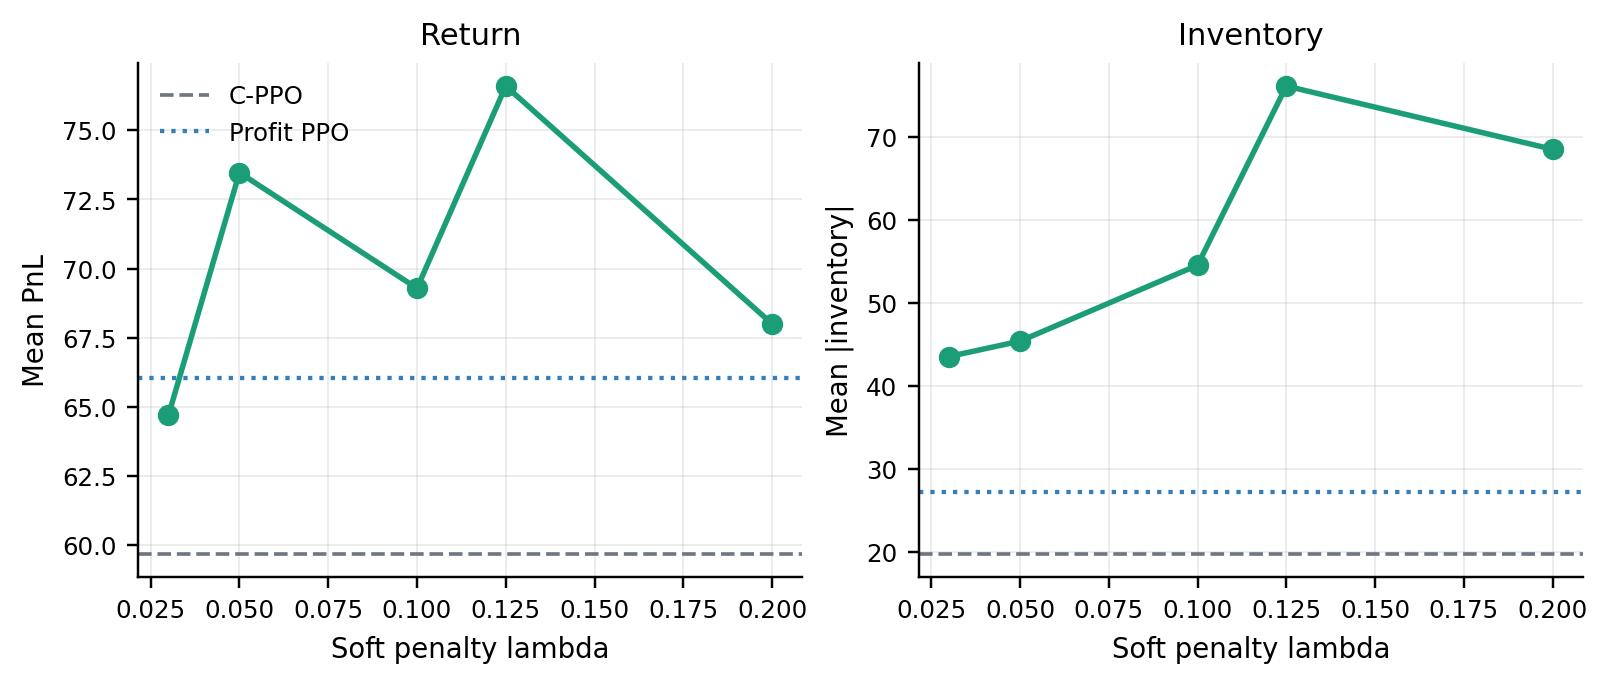
\includegraphics[width=0.92\textwidth]{figs/fig_lambda_sensitivity.png}
\caption{Sensitivity of soft AS regularization to $\lambda$ in the original three-seed 400k sweep. The selected low-risk teacher is reported in the main paper; this plot shows that the base-teacher penalty weight has a broad useful region, while inventory generally rises with tighter quoting.}
\label{fig:lambda}
\end{figure}

The broader matched sweep included base-teacher $\lambda\in\{0.03,0.05,0.10,0.125,0.20\}$, low-risk and high-risk teachers, fill-$\kappa$ calibration, hard AS windows, direct AS, and BC warm start. The selected main method uses the low-risk teacher with $\lambda=0.10$ because it gave the best balance of PnL, Sharpe, and behavioural alignment in the five-seed batch.

Hard AS applies the teacher as an action constraint rather than a training penalty: the PPO policy proposes an action, and the environment clips that action to a fixed window around the AS action before converting it to quotes. The wider hard window was the best hard-AS variant in the matched batch, but it still underperformed the selected soft regularizer. This is consistent with the role of the constraint. A hard window prevents the policy from taking large deviations even when the synthetic tape makes those deviations profitable. It also treats the AS teacher as locally correct at every step, which is too strong once the fill process, finite action bounds, and end-of-episode liquidation differ from the idealized AS assumptions. Hard AS is therefore useful as a guardrail diagnostic, but it is a less flexible way to combine the teacher with PPO.

BC warm start is different again. In the behavioural-cloning phase, the policy is trained by supervised learning to imitate AS actions on states from the training data; no RL reward is used in that phase. The resulting checkpoint is then fine-tuned with PPO using the pure-profit objective. This tests whether AS is best used only as an initialization. In exploratory runs it helped relative to training from scratch, but it was weaker than keeping the AS prior active during PPO. The likely reason is drift: once PPO fine-tuning begins, the policy can move away from AS without paying any continuing cost.

\section{Attention diagnostic}
\label{app:attention}

\begin{figure}[H]
\centering
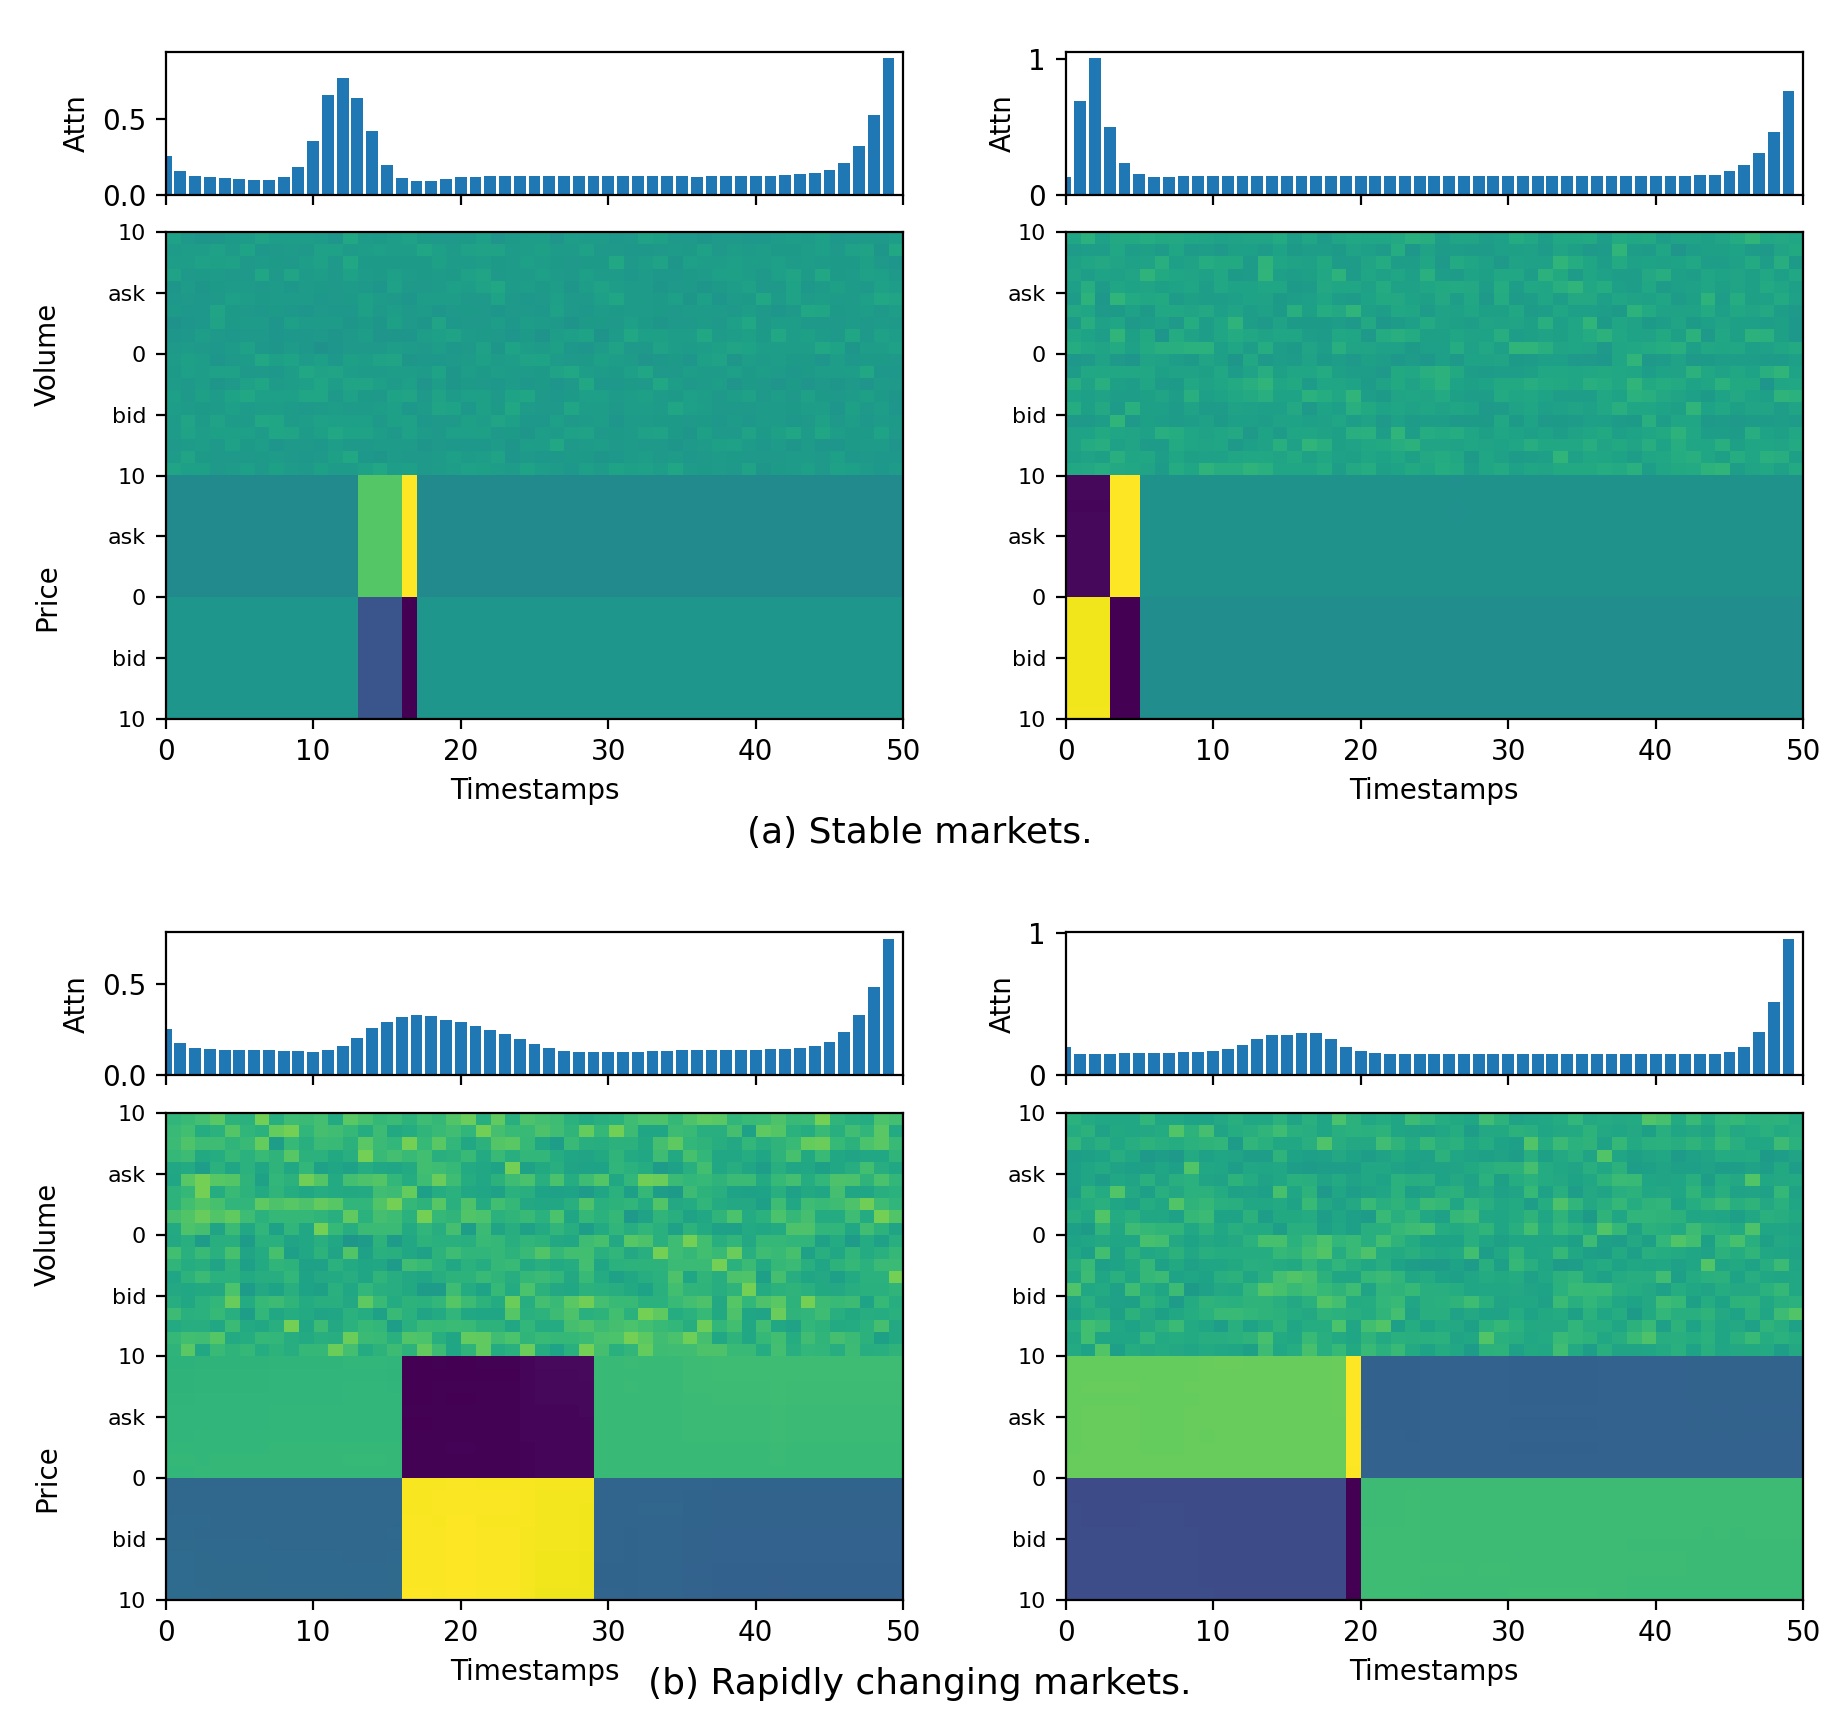
\includegraphics[width=0.78\textwidth]{figs/fig_attention.png}
\caption{Attention diagnostic for the proposed policy. Low-variation and high-variation windows are selected by mid-price standard deviation over the 50-event input window. The plot is included for comparison with the original paper's interpretability figure, but it should be read cautiously: attention maps are descriptive diagnostics, not causal explanations of trading performance.}
\label{fig:attention}
\end{figure}

The windows in Figure~\ref{fig:attention} are selected mechanically. For every possible 50-event input window, we compute the standard deviation of the level-1 mid-price. The two non-overlapping windows with the lowest values are labelled low-variation, and the two with the highest values are labelled high-variation. This makes the selection reproducible and matches the spirit of the original stable-versus-rapid comparison, but it is still a heuristic. We are confident that the selected windows differ in local mid-price variation under this metric; we should not claim that they are hand-validated economic regimes.

The upper panels show attention mass over the 50 input timestamps, aggregated from the Attn-LOB encoder's self-attention weights. The lower panels show the normalized LOB tensor for the same window. These heatmaps can look unusual because the LOB tensor is not an image: it stacks ask/bid prices and volumes across ten levels, with normalization applied per window. Persistent price ladders and large volume bands therefore appear as blocks or stripes. Attention can also look fairly flat after aggregation because different heads attend to different timestamps, and summing or averaging over heads smooths those patterns. In this run the diagnostic mainly says that the encoder is using broad recent context rather than placing a sharp, paper-like spike on a single event. That is informative, but weaker than the attention story in the original paper and should be treated as a qualitative check rather than evidence of mechanism.

\section{Per-stock numerical results}
\label{app:tables}

\begin{table}[h]
\centering
\small
\caption{Per-stock means over five seeds.}
\label{tab:perstock}
\begin{tabular}{llrrrr}
\toprule
Stock & Method & PnL & ND-PnL & Sharpe & Abs. inv. \\
\midrule
000001 & \cppo{} & $0.44$ & $8.0$ & $0.19$ & $0.5$ \\
000001 & \profitppo{} & $2.16$ & $44.3$ & $0.69$ & $2.2$ \\
000001 & \softas{} & $9.16$ & $282.7$ & $0.75$ & $64.2$ \\
000001 & Direct AS & $10.05$ & $363.4$ & $0.31$ & $214.8$ \\
000858 & \cppo{} & $172.64$ & $2292.5$ & $4.66$ & $52.1$ \\
000858 & \profitppo{} & $183.83$ & $2746.6$ & $4.38$ & $69.2$ \\
000858 & \softas{} & $190.92$ & $2689.4$ & $4.67$ & $62.4$ \\
000858 & Direct AS & $51.68$ & $517.6$ & $1.35$ & $52.0$ \\
002415 & \cppo{} & $7.15$ & $135.6$ & $1.36$ & $5.1$ \\
002415 & \profitppo{} & $11.02$ & $240.5$ & $1.81$ & $8.3$ \\
002415 & \softas{} & $25.44$ & $699.4$ & $2.20$ & $36.2$ \\
002415 & Direct AS & $18.18$ & $505.7$ & $0.58$ & $205.7$ \\
\bottomrule
\end{tabular}
\end{table}

\end{document}
